\chapter{Subastas y blockchain}\label{chapter:chapter1}

\hspace*{}

\section{Subastas}
  
  \hspace*{}

  Una subasta es el proceso de comprar y vender bienes o servicios. Este proceso implica ofrecer artículos 
  para vender, esperar que sean enviadas las ofertas y vender los bienes a la mayor oferta, bajo la supervisión
  de un subastador \parencite{krishna}.

  % An auction is a process of buying and selling goods or services. This process involves offering items 
  % for bidding, waiting for bids to be accepted, and then selling goods to the highest bidder under the 
  % supervision of an auctioneer. [5]

  Por la relevancia del término, se considera importante revisar qué definiciones formales de "subasta" existen:

  - Definición de la RAE: %(Real Academia Española)
  1. f. Venta pública de bienes o alhajas que se hace al mejor postor, y regularmente por mandato y con intervención de un juez u otra 
  autoridad.
  2. f. Adjudicación de una contrata, generalmente de servicio público, como la ejecución de una obra, el suministro de provisiones, etc., 
  a quien presenta la propuesta más ventajosa \parencite{raesubasta}.

  - Economipedia:
  Una subasta es un procedimiento de venta donde los interesados compiten entre sí para adjudicarse el bien o servicio a ser subastado 
  \parencite{economipediasubasta}.

  \subsection{Tipos de subastas} \hspace*{}

    Las subastas pueden clasificarse en diferentes tipos. A continuación se resumen las características de las más conocidas.

    - English Auction (Subasta Inglesa o ascendente): Este es el tipo de subasta más conocido. Las pujas comienzan con un precio bajo, y se 
    incrementan progresivamente a medida que se solicitan pujas más altas, hasta que se cierra la subasta o 
    no se reciben pujas más altas. A menudo el vendedor fija un precio de reserva por debajo del cual el 
    artículo no se vende y la subasta se cancela. Permite a un vendedor asegurar el precio más alto para un 
    artículo.

    - Dutch Auction (Subasta holandesa o descendente): El precio empieza alto y va bajando hasta que algún participante está 
    dispuesto a pagar el precio, y este es el que gana y paga el último precio que se menciona.

    \textbf{- Blind Auction (Subasta a ciegas o de sobre cerrado)}: También conocida en la literatura como First-Price sealed-bid auction(FPSBA)
    En este tipo de subasta, todas las ofertas se envían simultáneamente y nadie sabe que oferta hizo el resto
    de los participantes. Gana el que mayor oferta hizo y paga esa cantidad al vendedor.

    - Vickrey Auction (Subasta Vickrey): Conocida también en la literatura en inglés como sealed-bid second-price auction (SBSPA)
    % subasta de segundo precio de puja sellada
    . Es un tipo de subasta de puja sellada, donde los oferentes presentan ofertas por escrito sin conocer la oferta de las otras 
    personas en la subasta, y en la que gana el postor más alto, pero el precio que paga este es la segunda oferta más alta \parencite{economipediasubasta}.   
    % Este tipo de subasta fue descrito por primera vez por el profesor William Vickrey en la Universidad de Columbia en 1961 
    % % Vickrey, William (1961). «Counterspeculation, Auctions, and Competitive Sealed Tenders». The Journal of Finance 16 (1): 8-37. doi:10.1111/j.1540-6261.1961.tb02789.x.
    % , aunque había sido utilizada por coleccionistas de sellos desde 1893. Este tipo de subasta es estratégicamente similar a una 
    % subasta inglesa e incentiva a que los oferentes presenten ofertas iguales a su verdadera valoración del objeto subastado.
    % Las Subastas Vickrey son muy estudiadas en la literatura económica, pero no son particularmente comunes en la práctica.

    - All-pay auction (Subasta americana): es como la subasta inglesa, pero, todos los postores deben pagar la oferta que hacen, pero solo el que realiza 
    la mejor oferta obtiene el producto.
    % https://www.investopedia.com/terms/a/all-pay-auction.asp

    - Silent auction (Subasta Silenciosa):
    Las pujas se escriben en hojas de papel. Al final de la subasta, la puja más alta se adjudica la subasta. Este tipo de subasta se 
    utiliza frecuentemente en eventos de beneficencia, en los que se subastan muchos objetos simultáneamente, y se "cierra" a una hora 
    predeterminada común a todos los objetos. La subasta es "silenciosa" porque no hay subastador y los pujadores escriben sus pujas en 
    una hoja que usualmente se deja en una mesa cercana al objeto. En las subastas de beneficencia, las hojas usualmente indican una 
    puja inicial mínima, los incrementos que se pueden hacer sobre dicha puja mínima y una cantidad, llamada "puja garantizada" que si 
    se paga se obtiene el objeto de forma inmediata. Otras variaciones de este tipo de puja pueden incluir pujas selladas. El pujador 
    con la puja más alta paga el precio que indicó en su hoja y obtiene el bien \parencite{investopedia}.

    - Reverse auction (Subasta inversa o reversa):
    Es un tipo de subasta en la que se invierten los papeles de comprador y el vendedor. En una subasta ordinaria, los compradores compiten 
    para obtener un bien o servicio, ofreciendo precios cada vez más altos. En una subasta inversa, los vendedores compiten para obtener 
    negocio del comprador y los precios suelen disminuir a medida que los vendedores hacen sus ofertas.
      % https://es.wikipedia.org/wiki/Subasta_inversa

    - Candle Auction (Subasta de velas):
    Es una variación de la subasta típica inglesa que se hizo popular en los siglos XVII y XVIII. En una subasta de velas, el final 
    de la subasta se indica con el vencimiento de la llama de una vela, que tenía la intención de garantizar que nadie pudiera saber 
    exactamente cuándo terminaría la subasta y hacer una oferta de último segundo. A veces, se utilizaron otros procesos impredecibles, 
    como una carrera a pie, en lugar de la expiración de una vela \parencite{patten1970}.
    % https://en.wikipedia.org/wiki/Candle_auction

    - Double Auction (Subasta Doble):
    Una doble subasta es un proceso de compra y venta de bienes cuando los compradores potenciales y los posibles vendedores presenten 
    simultáneamente sus ofertas, su demanda, los precios de una casa de subastas, y luego un subastador elige algún precio \textit{p} que 
    equilibra el mercado: todos los vendedores que solicitaron menos de \textit{p} venden y todos los compradores que pujaron más de 
    \textit{p} compran a este precio \textit{p} \parencite{friedman1992}.
    % https://en.wikipedia.org/wiki/Double_auction
    
    Hay algunos otros tipos de subasta, pero mucho menos conocidas. Como fue explicado en la Introducción la presente investigación se 
    enfoca precisamente en subastas a ciegas.

  \subsection{Mercado de deuda} \hspace*{}

    El mercado de deuda o bonos es donde se emiten y negocian los títulos de deuda, cuando los participantes no están en condiciones o no 
    desean pedir préstamos o créditos a la banca. En él participan el Gobierno Federal, los gobiernos estatales o locales y las empresas 
    paraestatales o privadas que necesitan financiamiento, ya sea para realizar un proyecto de inversión o para mantener sus propias 
    actividades. Una parte de este mercado se conoce como mercado del dinero, que es en donde se intercambian los bonos que por su corto 
    plazo, liquidez y alta seguridad se pueden considerar sustitutos del dinero.

    El mercado de deuda también se conoce con otros nombres dependiendo del tipo de instrumentos de deuda negociado. Por ejemplo, si en el 
    mercado se negocian principalmente instrumentos de deuda que pagan una tasa fija, entonces se denomina mercado de renta fija, mercado 
    de renta variable, mercados de deuda internacional, de deuda pública, etc. En términos generales, para que una persona pueda comprar 
    o vender títulos de deuda es necesario que acudan a un banco o a una casa de bolsa para que dichas instituciones puedan efectuar las 
    transacciones necesarias a nombre de esta persona \parencite{bancomexico}.

    En este caso vamos a estar refiriéndonos específicamente al mercado de deuda pública o el mercado de bonos del Estado. Un bono del 
    Estado es un tipo de inversión basada en deuda, en que le prestas dinero a un gobierno a cambio de una tasa de interés acordada. Los 
    gobiernos los utilizan para generar fondos que pueden gastar en nuevos proyectos o infraestructura, mientras que los inversores 
    pueden usarlos a fin de que se les pague un retorno establecido en intervalos periódicos.

    Cuando compras un bono del Estado, le prestas al Gobierno una cantidad acordada de dinero durante un período también acordado. A 
    cambio de esto, el Gobierno te devuelve el dinero con un nivel establecido de interés de forma periódica, lo que se conoce como 
    cupón. De esta manera, los bonos conforman un activo de ingreso fijo.

    Cuando el bono venza, se te devolverá tu inversión original (denominada principal). El día en que recibes el valor de capital 
    adeudado se conoce como la fecha de vencimiento. Diferentes bonos tienen distintas fechas de vencimiento; por ejemplo, puedes 
    comprar un bono que vence en menos de un año o uno que vence en 30 años o más.

    Algunos inversores dicen que los bonos del Estado son inversiones libres de riesgo. Dado que un gobierno siempre puede imprimir más 
    dinero para saldar sus deudas, teóricamente hablando, siempre se te devolverá tu dinero cuando venza el bono.

    En la realidad, esto es mucho más complicado. En primer lugar, los gobiernos no siempre pueden producir más capital. Incluso si es 
    que pudieran hacerlo, esto no evita que incumplan el pago de los préstamos. No obstante, aparte del riesgo crediticio, existen otros 
    posibles problemas de los cuales preocuparse con los bonos del Estado, por ejemplo, el riesgo de las tasas de interés, la inflación 
    y las divisas \parencite{igbonos}.

  \subsection{Mercado de Deuda Pública en Cuba} \hspace*{}

    Cuando en nuestra economía doméstica los gastos superan a los ingresos no nos queda más remedio que pedir prestado, de lo contrario 
    no podemos pagar lo que necesitamos o debemos. En otras palabras, tendríamos que disminuir o aplazar las compras. Al presupuesto del 
    Estado le sucede exactamente lo mismo y sus ausencias de dinero se llaman déficit fiscal. La deuda pública es la suma del déficit 
    fiscal del año, más las garantías que se activen en esos 12 meses (porque el presupuesto del Estado es garante de determinadas 
    operaciones económicas como inversiones en sectores priorizados) y las amortizaciones de deudas anteriores provenientes de los bonos 
    que se colocaron en lo años anteriores.

    Pero, ¿cómo se financia el déficit presupuestario? Esto ocurre mediante bonos soberanos de la República de 
    Cuba que emite el Ministerio de Finanzas y Precios (MFP) y que hasta el momento han sido adquiridos por el sistema bancario nacional.

    El Banco de Inversiones es el encargado de colocar, emitir y registrar la emisión. El MFP le solicita una emisión de bonos y este lo 
    coloca en el sistema bancario, y cada banco comercial (Banco de Crédito y Comercio, Popular de Ahorro y Metropolitano) adquiere el 
    monto que puede asumir. En caso de que los bancos no tengan suficiente liquidez para cubrir totalmente el bono, interviene el Banco 
    Central de Cuba(BCC) con la emisión de nuevos billetes.

    Hasta 2013 el déficit se financiaba solo de esta manera (con la emisión de monedas por el BCC), pero debido a la inflación que 
    provoca el exceso de dinero en circulación se instrumentó los bonos soberanos y siempre se busca que la participación del BCC sea 
    en última instancia, porque es un dinero que se pone en circulación sin respaldo productivo \parencite{carmona2021}. 

    A pesar de que ya desde 2014 estan siendo emitidos los títulos de deuda soberana y de que legalmente
    es posible transar estos valores, la inexistencia de incentivos que promuevan la
    demanda de los títulos públicos y de condiciones básicas institucionales y de
    infraestructura del mercado han condicionado que las primeras colocaciones de bonos
    se hayan realizado mediante asignaciones administrativas. Lo cual demuestra que no
    resulta suficiente con emitir los títulos, si ello no se acompaña de transformaciones y
    reformas institucionales, estructurales, normativas y regulatorias que permitan ordenar,
    organizar e incentivar el funcionamiento de un Mercado de Deuda Pública. El sistema empleado hasta ahora
    esta muy lejos de ser el ideal. Para profundizar en este tema, se puede usar \parencite{barcelo2017}.

    Por parte del Instituto de Criptografía se desarrolla para el Banco Central de Cuba una plataforma para el Mercado de Deuda Pública de 
    Cuba. Una de las propuestas a utilizar en esta plataforma es una variación de la subasta holandesa(como se utiliza en casi todo el 
    mundo), pero en este caso, a ciegas sobre una blockchain, específicamente la blockchain de Quorum \ref{dutch_auction}.

    \begin{figure}[H]
      \center
      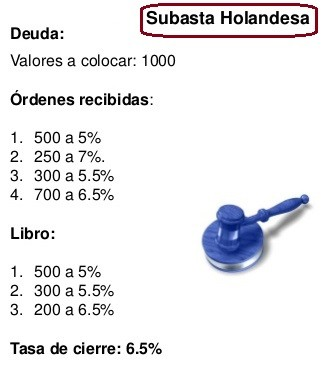
\includegraphics[scale=0.7]{photos/subasta-holandesa1.jpg}
      \caption{Ejemplo de subasta holandesa en el mercado de deuda}
      \label{dutch_auction}
    \end{figure}

\section{Blockchain} \hspace*{}
  Las subastas tradicionales usualmente requieren una tercera persona, ya sea un subastador o una 
  casa de subastas que maneje el proceso completo de subasta, lo cual puede llegar a tener muy altos
  impuestos por comisiones. También sufren de un punto de fallo, los subastadores pueden en ocasiones 
  tener malas intenciones \parencite{wu2019}. En este contexto, blockchain surge como una plataforma descentralizada que
  puede ser empleada para aplicaciones de subastas en línea confiables. En 2018 por primera vez en el 
  mundo una colección de arte valuada en varios millones de dólares perteneciente a Andy Warhol fue tokenizada
  y subastada satisfactoriamente usando la blockchain de Ethereum\parencite{wood2021}\parencite{emem}. Es también
  conocido que una de las mayores casas de subastas (e.g., Sotheby’s and Christie’s) está activamente
  trabajando en aplicar blockchain para subastas seguras y confiables. \parencite{neuendorf2018}

  % On the one hand, traditional centralized auctions usually require a third-party auctioneer or auction 
  % house to manage the entire auction process, which is expensive due to high commission fees. They also 
  % suffer from a single point of failure, as auctioneers can potentially be malicious in some cases [11]. 
  % In this context, blockchain has emerged as a decentralized platform to support trustworthy online 
  % auction applications. In 2018, for the first time in the world, multi- million dollar artworks by Andy 
  % Warhol were tokenized and auctioned successfully using the Ethereum blockchain [12],[13]. It is also 
  % reported that major auction houses (e.g., Sotheby’s and Christie’s) are actively working on applying 
  % blockchain in secure and trusted auction use cases [14].

  La tecnología blockchain elimina efectivamente los intermediarios, por lo tanto, reduce los costos de 
  transacción y asegura la confianza entre las partes interesadas en la subasta. En general, la tecnología
  blockchain puede mejorar las subastas en los siguientes aspectos:
  
  - Inmutabilidad de las transacciones de la subasta. Cada transacción ejecutada en la blockchain es pública, verificable e inmutable.
  Esto significa que la blockchain puede ser empleada como dispositivo de certificado de auditoría que previene que los participantes
  hagan trampa durante la subasta. El ganador puede usar la blockchain como prueba de la transacción.
  
  - Automatización del proceso de subasta. Un contrato inteligente automatiza el proceso de la subasta en la blockchain. Casi toda 
  la lógica de la subasta puede ser predefinida en contratos inteligentes para facilitar el intercambio de bienes y servicios, así como
  el pago de los tokens.

  - Descentralización del manejo de la subasta. No hay necesidad de designar una tercera persona como subastador, que asegure la 
  confiabilidad. Las tradicionales subastas centralizadas pueden ser muy costosas y sujeta a posibles subastadores tramposos; casas
  de subastas típicamente cargan del 8 al 20\% como comisión. 

  - Flexibilidad en el pago de la subasta. Las criptomonedas existentes en la blockchain pueden mejorar la seguridad y flexibilidad
  del pago de la subasta. Al mismo tiempo, un sistema de pago descentralizado, no necesita de intermediarios financieros, haciendo
  las transacciones más convenientes y menos costosas. \parencite{shi2021} %page 6

  \subsection{Quorum} \hspace*{}

    Blockchain es de los términos más usados en el mundo de la tecnología en estos días. Mientras esta tecnología es el elemento núcleo 
    de las criptomonedas que están llegando a los mercados financieros, su uso no es limitado a las criptos y tiene muchos más casos de uso.
    Con el pasar de los años, diferentes plataformas blockchain han sido desarrolladas con sus propios mecanismos de consenso y métodos de
    encriptación.

    Una de estas plataformas es la blockchain de Quorum, la cúal ha ganado popularidad en los últimos tiempos. Esto es a causa de la larga
    lista de casos de uso que quorum provee a sus usuarios. La red de Quorum está basada en una bifurcación de la blockchain de Ethereum.
    Es un protocolo blockchain de \href{https://github.com/ConsenSys/quorum}{código abierto} especialmente diseñado para usar en redes blockchain privadas. Algo a destacar de esta red
    es su nueva característica llamada \textit{"private transaction identifier"}  que asegura la privacidad de los datos. El objetivo de
    construir Quorum es utilizar la tecnología existente tanto como sea posible. Por lo tanto, incluso si la red Ethereum se somete a 
    diferentes actualizaciones en el futuro, habría pocos o ningún cambio en la blockchain de Quorum para mantener la sincronización entre
    estas redes. 
    % https://www.lcx.com/a-guide-to-quorum-blockchain/

    % Quorum fue creada por el super banco JPMorgan Chase, pero en 2020 fue adquirida la plataforma por ConsenSys empresa de tecnología de
    % sofware blockchain fundada por Joseph Lubin y con sede en la ciudad de New York. Por esa razón en ocasiones se le llama a la 
    % blockchain como ConsenSys Quorum
    % https://www.coindesk.com/business/2020/08/25/consensys-acquires-jpmorgans-quorum-blockchain/

  \subsection{Subastas a ciegas sobre blockchain} \hspace*{}
    Las subastas sobre blockchain han sido una área centro de muchas investigaciones en los últimos años.
    Razón por la cual ya se han desarrollado algunos protocolos de subastas a ciegas sobre 
    blockchain. Algunos de los cuales son:

    - \cite{hawk2016}

    - \cite{blass2017strain}

    - \cite{galalyusef2018}

    - \cite{sanchez2020}

    - \cite{sharma2021}

    - \cite{li2021}
